\chapter{Africa as a Natural Experiment}
\label{ch:africa}

\section{A continent of transplanted law}

At the Berlin Conference of 1884 and 1885 and in the decades that followed, European powers divided Africa among themselves along lines that often cut across existing political, ethnic and economic boundaries. Each colonial power brought its own law. British colonies received the common law, statutes of general application and English procedure, administered alongside customary law through systems of indirect rule. French colonies received the Napoleonic codes and French administrative law, administered more directly. Belgian, Portuguese, German, Spanish and Italian colonies received their own versions of civil law. In southern Africa, Roman Dutch law, the law of the Cape Colony before British rule, persisted as a mixed system. Islamic law governed personal matters, and in places criminal matters, across the Sahel and the north. Customary law, in hundreds of local varieties, continued to govern land, marriage and succession for most of the population.\index{Africa!legal systems}

Independence, mostly in the 1950s and 1960s and later in Portuguese and southern Africa, left these systems largely in place. Ghana, Nigeria, Kenya, Uganda, Tanzania, Zambia and Sierra Leone remained common law countries; Senegal, C\^ote d'Ivoire, Mali, Burkina Faso, Niger, Gabon and others remained civil law countries; South Africa, Botswana, Zimbabwe, Namibia and Lesotho retained mixed systems. This history makes Africa, as many scholars have noted, a natural laboratory for the legal origins thesis of Chapter~\ref{ch:llsv}. Neighbouring countries with similar geography, peoples and pre colonial institutions received different legal systems for reasons that had little to do with local conditions. If legal origin matters for economic outcomes, Africa is where we should be able to see it most clearly.

The laboratory is imperfect. Colonial powers differed in much besides law: in their education policies, their use of indirect rule, their investment in infrastructure, their treatment of missionaries, their extraction of resources and their exit. Separating law from everything else that came with it is the central challenge, and it is a problem of Bayesian inference with confounding \citep{klerman2011}.

\section{Borders as experiments}

\subsection{The idea}

When a colonial border divides a homogeneous area, the populations on either side were similar before colonisation and differ afterwards mainly in what the colonisers did. Comparing outcomes close to the border, where geography and pre colonial institutions are nearly identical, isolates the effect of colonial rule. This is a regression discontinuity design: outcomes are modelled as smooth functions of distance from the border, with a jump at the border measuring the effect.\index{regression discontinuity}

Michalopoulos and Papaioannou used the partition of ethnic homelands by colonial borders to study the effects of national institutions on development across Africa. They found that within partitioned ethnic homelands, differences in national institutions on either side of a border had surprisingly little effect on local economic development except near the capitals, measured by night time light density \citep{michalopoulos2014}, while in companion work they found that pre colonial ethnic institutions are strongly associated with development today \citep{michalopoulos2013}. Their result is a caution for any theory that attributes African development mainly to national institutions inherited from colonisers.

\subsection{Cameroon}

Cameroon offers the sharpest experiment, because the border runs inside a single country. Germany colonised Kamerun in the 1880s. After the First World War Britain and France divided it, and the League of Nations confirmed the division as a larger French mandate and a smaller British mandate along the Nigerian border. At independence in 1960 and 1961 the French territory and the southern part of the British territory united to form a federal republic, later a unitary state. The Anglophone regions in the north west and south west retained the common law, English language courts and English procedure; the Francophone regions retained the civil law. The country is bijural.\index{Cameroon}

Lee and Schultz used the former boundary between the British and French mandates as a discontinuity, comparing rural areas on either side within a single country, so that national institutions after reunification are held fixed \citep{lee2012}. They reported that areas on the formerly British side had higher levels of some measures of household wealth and access to public goods such as piped water. Figure~\ref{fig:rd} illustrates the design with simulated data. The design separates colonial legacy from national policy, but it cannot separate law from the other legacies of British rule, such as language, education and local administration. A difference at the border is the effect of the colonial package.

\begin{figure}[t]
\centering
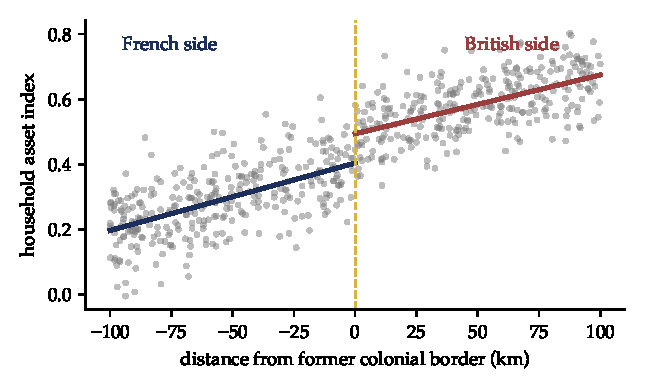
\includegraphics[width=\linewidth]{fig_rd}
\caption{A regression discontinuity across a former colonial border, with simulated data. The estimated jump at the border is the effect of the colonial package, of which the legal system is one component.}
\label{fig:rd}
\end{figure}

\subsection{A Bayesian border model}

A Bayesian analysis of border designs adds three things. First, it represents uncertainty about the functional form of the outcome as a function of distance, for instance with a flexible prior over smooth functions (a Gaussian process), so that the estimated jump does not depend on an arbitrary choice of polynomial. Second, it pools information across many borders with a hierarchical model, so that the effect at each border is estimated with the help of the others and the average effect of, say, British versus French rule is estimated with appropriate uncertainty. Third, it carries the uncertainty in each step through to the decomposition of the effect, using auxiliary data, into components attributable to different channels.

Let $y_{bi}$ be the outcome for location $i$ near border $b$, $x_{bi}$ its signed distance from the border, and $z_{bi}$ an indicator for the British side. A model is
\begin{equation}
y_{bi} = f_b(x_{bi}) + \delta_b z_{bi} + \epsilon_{bi}, \qquad \delta_b \sim N(\delta_0 + \gamma^\top w_b, \tau^2),
\label{eq:bordermodel}
\end{equation}
where $f_b$ is a smooth function, $\delta_b$ the jump at border $b$, $w_b$ border level covariates such as the difference in colonial education spending or in the share of indirect rule, and $\gamma$ their effects on the jump. If, after accounting for $w_b$, the residual jump $\delta_0$ is near zero, the evidence attributes the colonial effect to the measured channels rather than to law as such. If a legal variable, such as the presence of common law courts, has a large coefficient in $\gamma$, that is evidence for a legal channel.

\section{OHADA: harmonised business law}

In 1993, at Port Louis in Mauritius, a group of mainly Francophone African states signed a treaty establishing the Organisation for the Harmonisation of Business Law in Africa, known by its French acronym OHADA. Its members, now seventeen states mostly in West and Central Africa, adopt uniform acts that apply directly in each member state on subjects including general commercial law, company law, secured transactions, debt recovery, insolvency, arbitration and accounting. A Common Court of Justice and Arbitration in Abidjan serves as the supreme court for questions arising under the uniform acts, displacing national supreme courts in those matters.\index{OHADA}

OHADA is one of the largest experiments in legal harmonisation outside Europe. Its premise is that investors are deterred by fragmented, outdated and unpredictable business law, and that a single modern code applied by a common court would reduce uncertainty. In the terms of Chapter~\ref{ch:commoncivil}, OHADA strengthened the prior: it replaced many national rules with one set, and it created a court whose decisions accumulate across states, so that precedent, though formally not binding, is pooled. A hierarchical model of how courts apply the uniform acts would treat each state's courts as a group, with partial pooling toward the common court's interpretations.

Cameroon is an OHADA member, which raised a difficult question for its Anglophone regions: uniform acts drafted in the French civil law tradition had to be applied by common law courts. English translations of the acts were initially unavailable or unofficial, and common law lawyers objected to applying a civil law code in a common law jurisdiction. The tension was one strand of a wider grievance.

\section{The Anglophone crisis and the courts}

In late 2016 lawyers in Cameroon's Anglophone regions went on strike, protesting among other things the appointment of Francophone magistrates trained in the civil law to courts in the common law regions, the use of French in court proceedings there, and the failure to provide official English versions of OHADA acts. Teachers joined with parallel grievances about education. The protests were met with force, and the conflict escalated into an armed separatist insurgency and a humanitarian crisis that has continued for years.\index{Anglophone crisis}

The government's responses included the creation in 2017 of a common law division within the Supreme Court and, in 2018, a common law section at the national school for magistrates. These were attempts to preserve the bijural system by strengthening the institutions of the minority tradition. Whatever one thinks of the wider political conflict, its legal origins illustrate a point that cross country regressions cannot capture: legal systems are not only rules but communities of practitioners with shared training, language and expectations. A judge trained in one tradition, applying the procedural intuitions of that tradition in a court of the other, produces decisions that the parties perceive as illegitimate. In Bayesian terms, the judge's prior about how evidence should be presented and weighed does not match the parties', and the resulting decisions have high variance relative to what the parties can predict.

\section{Customary law and evidence}

For most Africans, customary law governs the most important matters in their lives: access to land, marriage, inheritance and the resolution of local disputes. British colonial regimes recognised customary law subject to a repugnancy clause, under which customs repugnant to natural justice, equity and good conscience would not be enforced. Post independence constitutions generally recognise customary law subject to fundamental rights.\index{customary law}

Customary law poses a distinctive evidence problem. Its content is not written in a code or in reported cases but held in the memory of elders and communities. In many jurisdictions courts must find it as a matter of fact, through the testimony of experts or assessors, unless it is notorious enough for judicial notice; a few, such as Ghana, treat it as a question of law. In Bayesian terms, the content of a customary rule is an unknown parameter about which the court receives noisy testimony, and the testimony may be shaped by the interests of the witnesses, since the rule on, say, women's inheritance rights affects who receives land. A coherent approach would treat each witness's account as a signal with an estimated reliability and a possible bias, and combine them as in Chapter~\ref{ch:graphs}, with the court mindful that the most authoritative witnesses may be those with the greatest stake.

\section{Election petitions: evidence at the highest stakes}

African courts have been asked to decide some of the highest stakes evidential questions any court faces: whether a presidential election was conducted so irregularly that it must be annulled. In September 2017 the Supreme Court of Kenya annulled the presidential election of the previous month, finding that the electoral commission had failed to conduct it in accordance with the constitution and the law, in particular in the transmission and verification of results. It was widely reported as the first time a supreme court in Africa had annulled a presidential election. In February 2020 the Constitutional Court of Malawi annulled the 2019 presidential election on the basis of widespread irregularities, and the Supreme Court of Appeal upheld the decision; the rerun election was won by the opposition candidate.\index{election petitions}

These cases raise in sharp form the questions of this book. What is the standard of proof for annulment? Most courts require the petitioner to show irregularities that affected the result, or that the conduct of the election so departed from the law that its result cannot be trusted. The first is a counterfactual question: would the result have been different without the irregularities? The second is a question about the integrity of a process. A Bayesian analysis of the first would model the vote counts at each polling station, the probability and size of irregularities, and the resulting uncertainty about the margin. If the margin is large relative to the plausible effect of irregularities, the posterior probability that they changed the result is small. If the margin is narrow, or the irregularities are widespread and unquantifiable, the posterior may be close to one half, and the decision must turn on the relative losses (the threshold of \eqref{eq:threshold}) of annulling a valid result and confirming an invalid one. Statistical methods for detecting anomalies in election returns, such as tests on the distribution of digits or of turnout and vote shares, are evidence of irregularity, but each has false positive rates that a court must understand.

The Kenyan and Malawian courts reasoned primarily about process: whether the law had been followed. A process based standard has the advantage that it does not require the court to estimate a counterfactual vote count, which may be impossible. It has the disadvantage that it can annul elections whose results were not in doubt. The decision theoretic framework does not choose between these standards, but it shows what each implies about the losses the court is weighing.

\section{Courts, contracts and development}

The \emph{Courts} study of Chapter~\ref{ch:llsv} \citep{djankov2003} found that procedural formalism is higher in civil law countries and associated with slower and less consistent decisions. Many African countries, both common law and civil law, have slow courts and large backlogs. For a small business, the expected value of a contract claim is the probability of winning times the amount, minus costs, discounted for delay. If a commercial case takes several years to resolve, the discounted value of a claim may be small, and the threat of litigation provides weak incentives to perform. Businesses respond by contracting only with those they know, relying on reputation and relationships rather than courts, which is the subject of Chapter~\ref{ch:gould}.

Technology offers some hope. Several African judiciaries have introduced electronic case management, filing and virtual hearings, especially since the pandemic. Specialised commercial courts, small claims procedures and arbitration centres aim to provide faster resolution for commercial disputes. The question for evaluation is whether these reforms change the posterior that a businessperson holds about the likely outcome and timing of a dispute, and thereby change behaviour. Randomised and quasi experimental evaluations, analysed with hierarchical Bayesian models that pool across courts and countries, are the natural tool.

\section{Lessons}

Africa shows that legal origin is one of many colonial legacies, and that its effects cannot be read off cross country regressions. Border designs isolate colonial effects but not the legal component of them. Bijural states such as Cameroon show that legal systems are communities of practice, and that the coexistence of traditions requires institutions that respect both. OHADA shows the attractions and the difficulties of harmonisation. Customary law and election petitions pose evidential problems of their own. Throughout, a Bayesian approach clarifies what the evidence can and cannot establish and what decisions under uncertainty require.

\section*{Notes and Questions}
\addcontentsline{toc}{section}{Notes and Questions}
\begin{enumerate}[label=\arabic*.]
\item In the border model \eqref{eq:bordermodel}, suppose there are ten borders with estimated jumps and standard errors of your choice. Compute the partially pooled estimates and the posterior for $\delta_0$ under a normal prior, treating $\tau$ as fixed and then as given a prior of your choice.
\item Lee and Schultz compare areas within Cameroon. What advantages does this have over comparing Nigeria and Cameroon at their international border? What does it not control for?
\item Design an evidentiary procedure for finding the content of a customary rule of inheritance, given that the most knowledgeable witnesses may have an interest in the outcome.
\item In a presidential election with ten million votes cast and a winning margin of two hundred thousand, irregularities are found at five per cent of polling stations. Under what assumptions about the size and direction of the irregularities would the posterior probability that they changed the result exceed one half?
\item OHADA's uniform acts apply directly in member states and are interpreted by a common court. In what sense does this pool precedent? What are the risks for a common law region within a member state?
\item Is a process based standard for annulling elections better than an outcome based standard? Answer in terms of the losses from each kind of error.
\end{enumerate}

\section*{Further reading}
Michalopoulos and Papaioannou on national institutions and partitioned ethnic groups \citep{michalopoulos2014}; Lee and Schultz on Cameroon \citep{lee2012}; Klerman and colleagues on colonial history \citep{klerman2011}.
